% Node Graph (Directed Graph)
% Demonstrates: node positioning, edge styles, labels, and graph layout.
% Compile with: pdflatex main.tex

\documentclass{article}
\usepackage{tikz}
\usetikzlibrary{arrows.meta, positioning}

\begin{document}
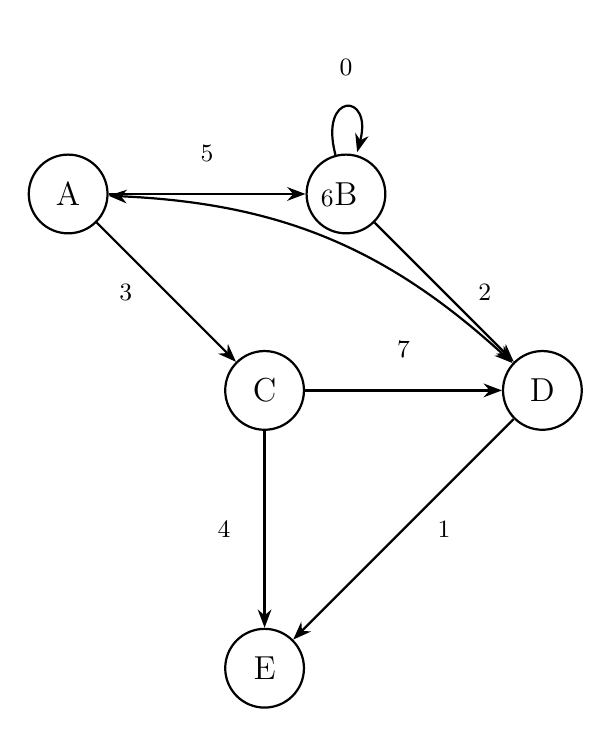
\begin{tikzpicture}[
    ->,
    >=Stealth,
    node distance=2.5cm,
    every node/.style={circle, draw, minimum size=1cm, font=\large},
    thick
]

% --- Nodes ---
\node (A) {A};
\node (B) [right=of A] {B};
\node (C) [below right=of A] {C};
\node (D) [right=of C] {D};
\node (E) [below=of C] {E};

% --- Edges with labels ---
\draw (A) -- node[above, draw=none, font=\small] {5} (B);
\draw (A) -- node[left, draw=none, font=\small] {3} (C);
\draw (B) -- node[right, draw=none, font=\small] {2} (D);
\draw (C) -- node[above, draw=none, font=\small] {7} (D);
\draw (C) -- node[left, draw=none, font=\small] {4} (E);
\draw (D) -- node[right, draw=none, font=\small] {1} (E);

% --- Self-loop ---
\draw (B) edge[loop above] node[draw=none, font=\small] {0} (B);

% --- Bidirectional edge ---
\draw[<->] (A) to[bend left=20] node[above, draw=none, font=\small] {6} (D);

\end{tikzpicture}
\end{document}
